\documentclass[12pt,a4paper]{article}
\usepackage{graphicx}
\usepackage{listings}
\usepackage{color}
\usepackage{pdfpages}
\definecolor{codegreen}{rgb}{0,0.6,0}
\definecolor{codegray}{rgb}{0.5,0.5,0.5}
\definecolor{codepurple}{rgb}{0.58,0,0.82}
\definecolor{backcolour}{rgb}{0.95,0.95,0.92}
 
\lstdefinestyle{mystyle}{
    backgroundcolor=\color{backcolour},   
    commentstyle=\color{codegreen},
    keywordstyle=\color{magenta},
    numberstyle=\tiny\color{codegray},
    stringstyle=\color{codepurple},
    basicstyle=\footnotesize,
    breakatwhitespace=false,         
    breaklines=true,                 
    captionpos=b,                    
    keepspaces=true,                 
    numbers=left,                    
    numbersep=5pt,                  
    showspaces=false,                
    showstringspaces=false,
    showtabs=false,                  
    tabsize=2
}
 
\lstset{style=mystyle}



\graphicspath{ {images/} }
\begin{document}
	\begin{titlepage}
		\title{data Structure project \\ phase1}
		\maketitle
		\begin{center}
			\author{Ali A. Taheri \\ Ehsan E. Vakhshoori}
		\end{center}
	\end{titlepage}
	\newpage
	\tableofcontents
	\newpage
	\section{time series and time series motifs}
	\section*{time series}
	‘Time’ is the most important factor which ensures success in a business. It’s  difficult to keep up with the pace of time.
	\\ A Time Series is a sequence $T=(t_{1} ,t_{2} ,...,t_{n} )$ which is an ordered set of n real valued numbers.
	\\ The ordering is typically temporal however other kinds of data such as color distributions shapes and spectrographs also have a well defined ordering and canfruitfully be considered “time series” for the purpose of indexing and mining.
	\\ \\ For example:
	\begin{itemize}
		\item{Monthly unemployment rates for the previous five years.}
		\item{Daily production at a manufacturing plant for a month.}
		\item{Decade-by-decade population of a state of the previous century.}		
	\end{itemize}
	Components of a time series
	\section*{Trend}
	The long-term tendency of a series to increase or fall (upward trend or downward trend).
	\section*{Seasonality}
	The periodic fluctuation in the time series within a certain period. These fluctuations form a pattern that tends to repeat from one seasonal period to the next one.
	\section*{Cycles}
	Long departures from the trend due to factors others than seasonality. Cycles usually occur along a large time interval, and the lengths of time between successive peaks or troughs of a cycle are not necessarily the same.
	\section*{Irregular movement}
	The movement left after explaining the trend, seasonal and cyclical movements; random noise or error in a time series.
	\section*{time series motifs}
	Time series motifs are pairs of individual time series, or subsequences of a longer time series, which are very similar to each other.
Time series motifs are repeated segments in a long time series that, if exist, carry precise information about the underlying source of the time series. Motif discovery in time series data has received significant attention in the data mining community since its inception, principally because, motif discovery is meaningful and more likely to succeed when the data is large.
	\section{difference between match and trivial match in a time series}
	\section*{match}
	Given a positive real number R (called range) and a time series T containing a subsequence C beginning at position p and a subsequence M beginning at q, if $D(C, M) \leq R$, then M is called a matching subsequence of C.
	\\ The first three definitions are summarized in Figure 2, illustrating a time series of length 500, and two subsequences of length 128.
	\section*{trivial match}
	Trivial Match: Given a time series T, containing a subsequence C beginning at position p and a matching subsequence M beginning at q, we say that M is a trivial match to C if either $p = q$ or there does not exist a subsequence M beginning at q such that dist$(C, M ) > R$, andeither $q < p$ or $p < q$.
	\begin{figure}[h]
		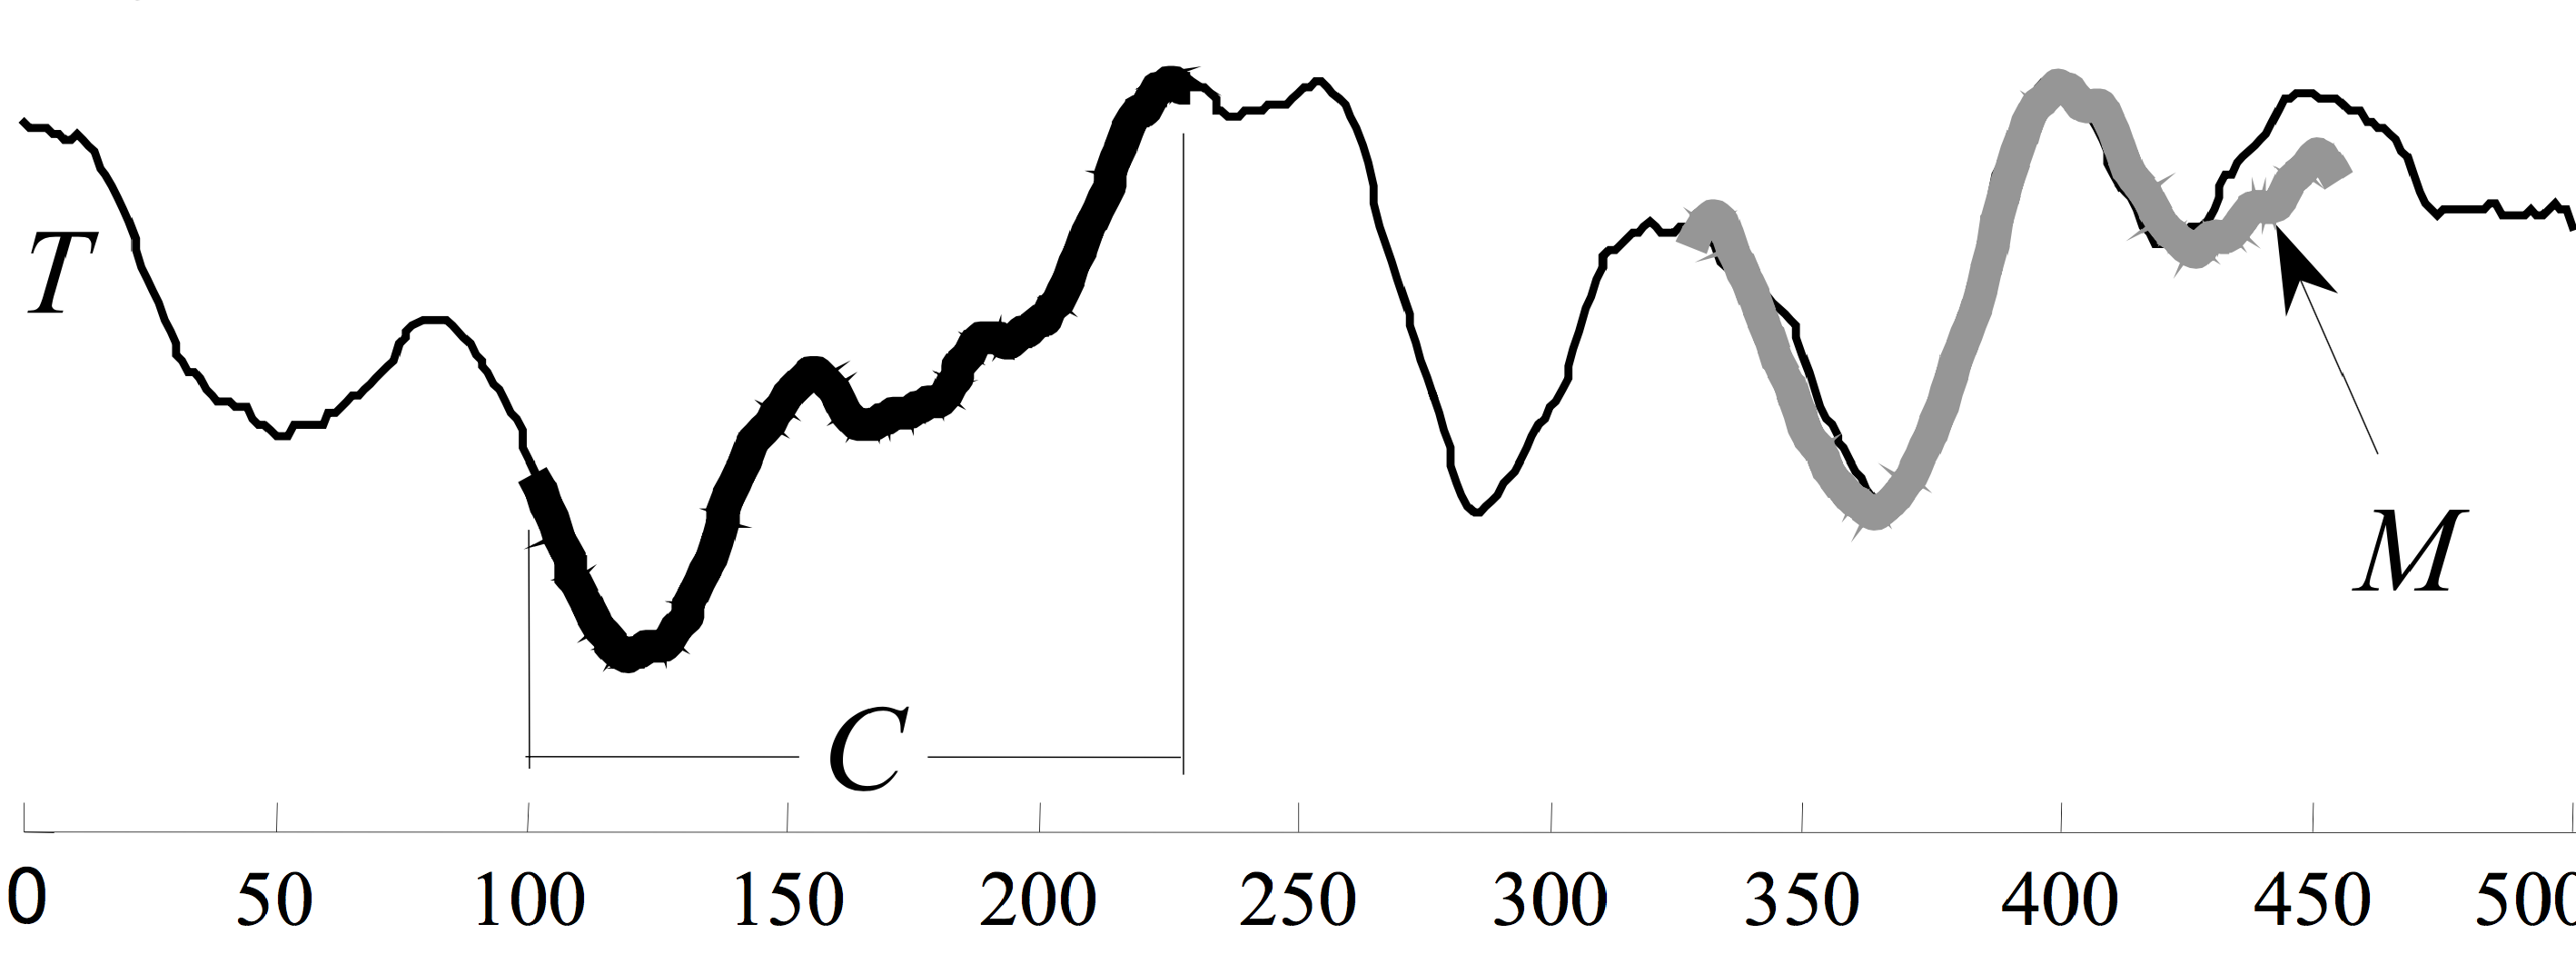
\includegraphics[width=\textwidth]{pic1.png}
		\caption{A visual intuition of a time series T (light line), a subsequence C
(bold line) and a match M (bold gray line)}
	\end{figure}
	\section{subsequence motif in a time series}
	Time series motifs are pairs of individual time series, or subsequences of a longer time series, which are very similar to each other.
	\\ The $k^{th}$-Time Series motif is the $k^{th}$ most similar pair in the database D. The pair $T_i$, $T_j$ is the $k^{th}$ motif iff there exists a set S of pairs of time series of size exactly k-1 such that $\forall t_b$ and $\{ t_j , t_d \} \in S$ and $\forall \{ t_x , t_y \} \in S$, $ \{ t_w , t_b \} \notin S$, $dist(t_x , t_y) \leq dist(t_i , t_j) \leq dist(t_a , t_b)$.
	\\ Instead of dealing with pairs only we can also extend the notion of motifs
to sets of time series that are very similar to each other.
	\\ The Subsequence Motif is a pair of subsequences $ \{ T_{i,n} , T_{j,n} \} $ of a long time series T that are most similar. More formally, $\forall a, b, i, j$ the pair $ \{ T_{i,n} , T_{j,n} \} $ is the subsequence motif iff $dist(T_{i,n} , T_{j,n}) \leq dist(T_{a,n} , T_{b,n}), |i-j| \geq w$ and $|a-b| \leq w$ for $w>0$.
	\\ Note that we impose a constraint on the relative positions of the subsequence 
in the motif. This says that there should be a gap of at least w places between the subsequences. This restriction helps to prune out the trivial subsequence motifs. For example (and considering discrete data for simplicity), if we were looking for motifs of length four in the string: sjdbbnvfdfpqoeutyvnABABABmbzchslfkeruyousjdq  Then in this case we probably dont want to consider the pair \{ABAB, ABAB\} to be a motif, since they share 50\% of their length (i.e AB is common to both). Instead, we would find the pair $ \{ sjdb, sjdq \} $ to be a more interesting approximately repeated pattern. In this example, we can enforce this by setting the parameter $w=4$. In all the definitions given above we assumed there is a meaningful way to measure the distance between two time series. There are several such ways in the literature and our method is valid for any distance measure that is a metric. We use Euclidean distance and express it as $d(A,B)$. Recently extensive empirical comparisons have shown that the Euclidean distance is completive with or superior to more complex measures on a wide variety of domains. Furthermore, its competitiveness increases as the datasets get larger, and it is large datasets that are of interest here.
	\begin{figure}[h]
	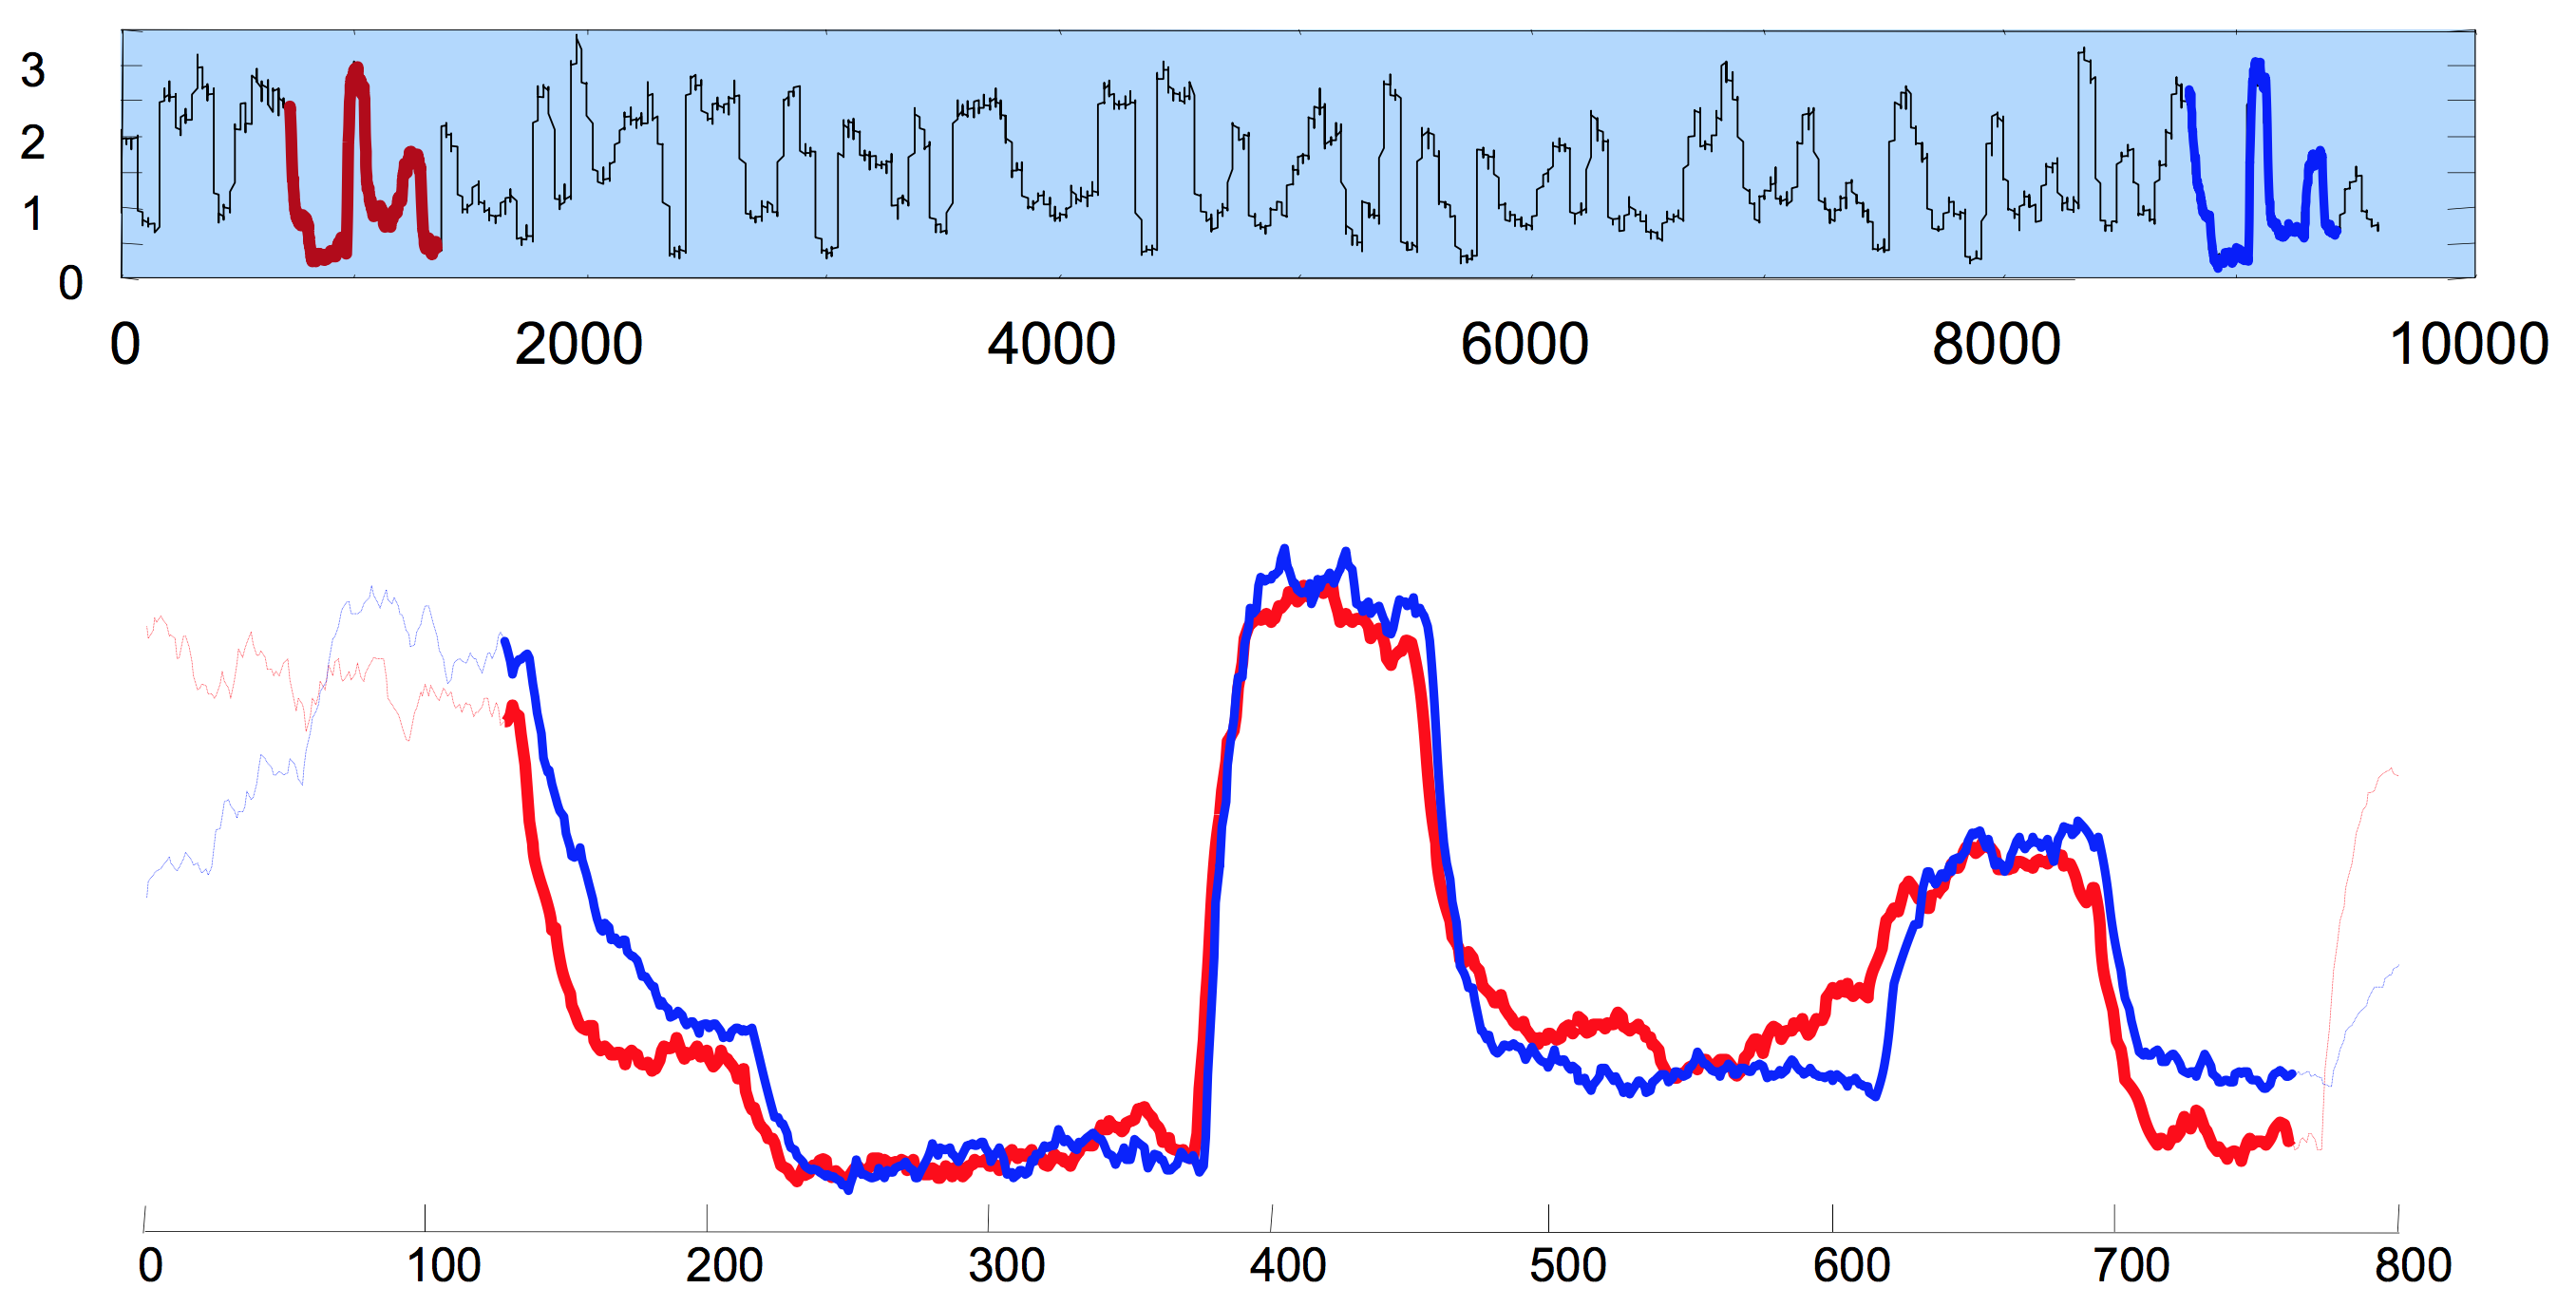
\includegraphics[width=\textwidth]{pic2.png}
	\caption{time motives}
	\end{figure}
	\section{datasets for time series}
	Generate some input for main algorithm with c++:
	\\ \\ (signal):
	\lstinputlisting[language=c]{MakeInput1.cpp}
	\pagebreak
	(string):
	\lstinputlisting[language=c]{MakeInput2.cpp}
	\section{algorithm to detect time series motifs}
	\lstinputlisting[language=python]{Code.py}
	\pagebreak
	\section{program’s output for a data}
	Input date: sjdbbnvfdfpqoeutyvnABABABmbzchslfkeruyousjdq
	\\ \\ output for this data with K=4 \& R=1 :
	\lstinputlisting{output(R=1).txt}
	output for this data with K=4 \& R=2 :
	\lstinputlisting{output(R=2).txt}
	output for this data with K=4 \& R=3 :
	\lstinputlisting{output(R=3).txt}
	\pagebreak
	\section{How much time it takes for algorithm to find motifs?}
	The brute force algorithm has a time complexity of $O(m^2)$.
	\\ This is critical because each distance computation takes $O(k)$ time
which makes the brute force algorithm an $O(k m^2)$ algorithm
	\begin{figure}[h]
		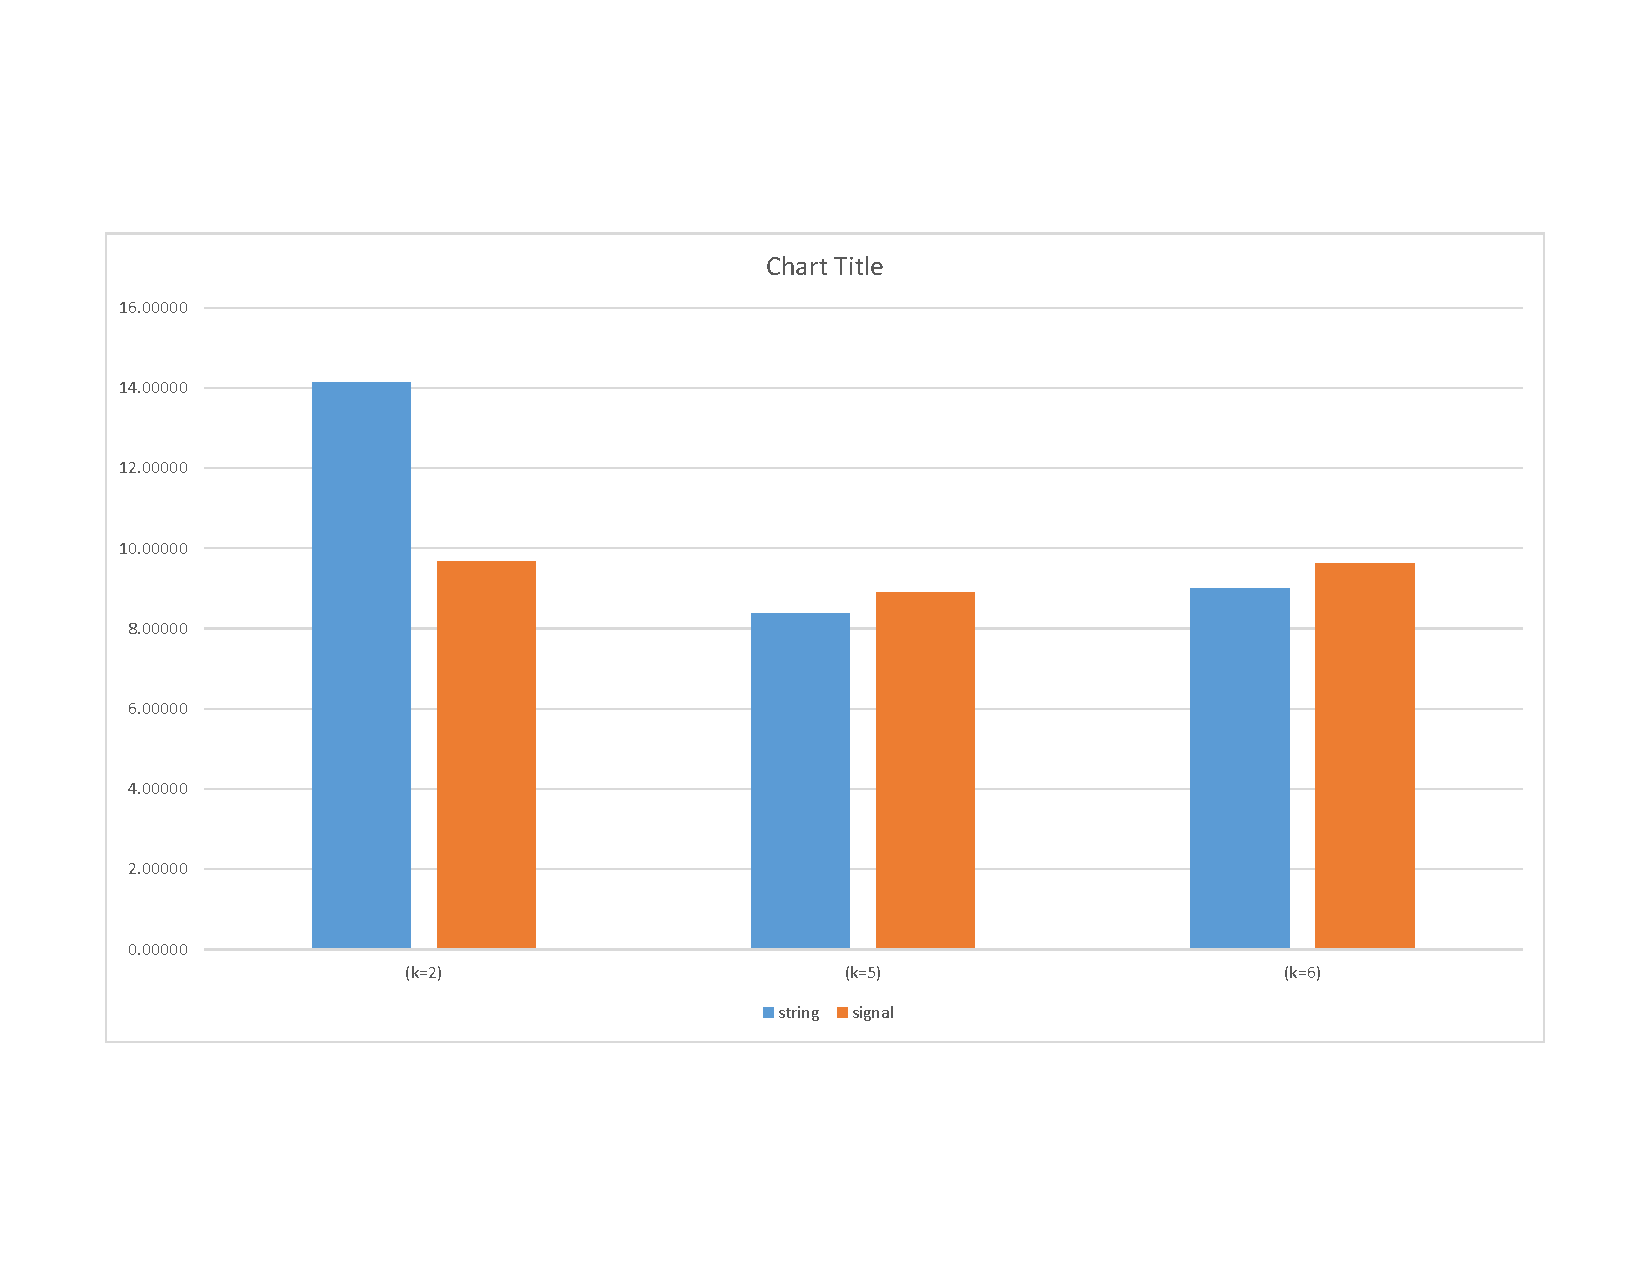
\includepdf[width=\textwidth]{Chart.pdf}
	\end{figure}
\end{document}
